\chapter[Aula 7]{Independência e Leis Zero-Um}
\chaptermark{}

\section{Expansões Diádicas de Números Aleatórios Distribuídos Uniformemente}

Apresentamos nesta seção outro exemplo interessante
de v.a.'s independentes. Desta vez nosso espaço 
de probabilidade será 
$(\Omega,\F,\P)=\Big((0,1],\mathscr{B}((0,1]),\lambda\Big)$,
onde $\lambda$ é a medida de Lebesgue em $(0,1]$.

Para definir a v.a.'s que estamos interessados,
precisamos fazer primeiro algumas observações. 
Para cada $\omega\in (0,1]$ existem
números $d_n(\omega)\in\{0,1\}$, com $n\in\N$  
tais que 
	\[
		\omega = \sum_{n=1}^{\infty} \frac{d_n(\omega)}{2^n}.
	\] 
Observamos que os números $d_n(\omega)$ na igualdade 
acima não são unicamente determinados por $\omega$. Por exemplo, 
para $\omega=1/2$ temos 
	\[
		\frac{1}{2} = \frac{0}{2^1}+\frac{1}{2^2}+\frac{1}{2^3}+\ldots
		\qquad
		\text{e}
		\qquad
		\frac{1}{2}= \frac{1}{2^1}+\frac{0}{2^2}+\frac{0}{2^3}+\ldots.
	\]  
Um fato importante é que este é o único tipo 
de não unicidade que ocorre na expansão diádica de um 
número no intervalo $(0,1]$. 
Este fato permite fazer uma escolha apropriada
de forma que $d_n:\Omega\to\{0,1\}$ seja de fato 
uma função. Esta escolha é feita da seguinte maneira:
sempre que $\omega$ admitir mais de uma 
expansão diádica, 
seja $d_n(\omega)$ o $n$-ésimo digito da expansão 
diádica de $\omega$ que termina em uma sequência 
infinita de uns consecutivos.
Esta escolha no exemplo acima determina uma 
única expansão diádica para $1/2$ que é dada por $d_1(1/2)=0$ e
$d_n(1/2)=1$, para todo $n\geq 2$.

\begin{proposicao}
	Para todo $n\in\N$ a função $d_n:\Omega\to\{0,1\}$ 
	como definida acima é uma variável aleatória. 
\end{proposicao}



\begin{proof}
Como $d_n$ assume apenas dois valores, 
para provar a proposição basta mostrar 
que 
	\[
		\{d_n=0\}\in\mathscr{B}((0,1])
		\qquad
		\text{e}
		\qquad
		\{d_n=1\}\in\mathscr{B}((0,1]),
	\]
para todo $n\in\N$.
Já que $\{d_n=0\} = \{d_n=1\}^c$, é suficiente
mostrar que $\{d_n=1\}\in \mathscr{B}((0,1])$.



Para ajudar na compreensão do argumento mostramos 
qual é a ideia da prova em um 
caso mais simples, onde $n=1$. Neste caso 
temos 
	\begin{align*}
		\{d_n=1\}
		&=
		\left(
		\frac{1}{2^1}+\frac{0}{2^2}+\frac{0}{2^3}+\ldots
		\right.
		\ \ \mathbf{,} \ \ 
		\left.
		\frac{1}{2^1}+\frac{1}{2^2}+\frac{1}{2^3}+\ldots
		\right]
		\\[0.3cm]
		&=
		\left(\frac{1}{2},1\right]
		\in \mathscr{B}((0,1]).
	\end{align*}
Observe que o intervalo acima é aberto no extremo esquerdo
por causa da escolha que fizemos da expansão e portanto 
$1/2\in \{d_1=0\}$.

Para $n\geq 2$ temos que 
	\begin{align*}
		\{d_n=1\}
		&=
		\bigcup_{(u_1,\ldots,u_{n-1})\in\{0,1\}^{n-1}}
		\left(
		\frac{u_1}{2^1}+\frac{u_2}{2^2}+\ldots+\frac{u_{n-1}}{2^{n-1}}+\frac{1}{2^{n}}
		+\frac{0}{2^{n+1}}+\frac{0}{2^{n+2}}+
		\ldots
		\right.
		\\
		&\qquad\qquad\qquad
		\ \ \mathbf{,} 
		\left.
		\frac{u_1}{2^1}+\frac{u_2}{2^2}+\ldots+\frac{u_{n-1}}{2^{n-1}}+\frac{1}{2^{n}}
		+\frac{1}{2^{n+1}}+\frac{1}{2^{n+2}}+
		\ldots
		\right].
	\end{align*}
O lado direito da igualdade acima é uma união 
disjunta de $2^{n-1}$ intervalos e portanto este
conjunto pertence a $\mathscr{B}((0,1])$.

Por exemplo, 
	\[
	\{d_2=1\} 
	= \left( \frac{1}{4},\frac{1}{2} \right]
	\cup 
	\left( \frac{3}{4},1  \right].
	\]
\end{proof}




\begin{proposicao}
	Para todo $n\in\N$ temos que $\lambda(\{d_n=1\})=1/2$.
\end{proposicao}



\begin{proof}
Usando a representação obtida na proposição acima e 
a aditividade de $\lambda$ temos que 
%
	\begin{align*}
		\lambda(\{d_n=1\})
		&=
		\lambda
		\left(		
			\bigcup_{(u_1,\ldots,u_{n-1})\in\{0,1\}^{n-1}}
			\left(
				\frac{u_1}{2^1}
				+\frac{u_2}{2^2}
				+\ldots+\frac{u_{n-1}}{2^{n-1}}+\frac{1}{2^{n}}
				+\frac{0}{2^{n+1}}+\ldots
			\right.
		\right.
		\\
		&\qquad\qquad\qquad
		\ \ \mathbf{,} 
		\left.
			\left.
				\frac{u_1}{2^1}+\frac{u_2}{2^2}
				+\ldots+\frac{u_{n-1}}{2^{n-1}}+\frac{1}{2^{n}}
				+\frac{1}{2^{n+1}}+\frac{1}{2^{n+2}}
				+\ldots
			\right]
		\right).
		\\[0.8cm]
%
%	SEGUNDA IGUALDADE
%
		&=
		\sum_{(u_1,\ldots,u_{n-1})\in\{0,1\}^{n-1}}
		\lambda
		\left(		
			\left(
				\frac{u_1}{2^1}
				+\frac{u_2}{2^2}
				+\ldots+\frac{u_{n-1}}{2^{n-1}}+\frac{1}{2^{n}}
				+\frac{0}{2^{n+1}}+\ldots
			\right.
		\right.
		\\
		&\qquad\qquad\qquad
		\ \ \mathbf{,} 
		\left.
			\left.
				\frac{u_1}{2^1}+\frac{u_2}{2^2}
				+\ldots+\frac{u_{n-1}}{2^{n-1}}+\frac{1}{2^{n}}
				+\frac{1}{2^{n+1}}+\frac{1}{2^{n+2}}
				+\ldots
			\right]
		\right)
		\\[0.8cm]
%
%	TERCEIRA IGUALDADE
%
		&=
		\sum_{(u_1,\ldots,u_{n-1})\in\{0,1\}^{n-1}}
		\sum_{k=n+1}^{\infty} \frac{1}{2^k}
		=
		\sum_{(u_1,\ldots,u_{n-1})\in\{0,1\}^{n-1}}
		\frac{1}{2^{n+1}(1-1/2)}
		=\frac{1}{2}.
	\end{align*}
\end{proof}

















\begin{proposicao}
A sequência $\{d_n\}$ é uma sequência de variáveis aleatórias iid no
espaço de probabilidade
$\Big((0,1],\mathscr{B}((0,1]),\lambda\Big)$.
\end{proposicao}


\begin{proof}
Já que $d_n$ assume apenas os valores $0$ e $1$ segue da
proposição anterior que $\{d_n\}$ é identicamente distribuída.
Portanto basta provar que esta sequência é independente. 
Para isto é suficiente mostrar que para todo $n\in\N$ 
as variáveis aleatórias $\{d_1,\ldots,d_n\}$ são independentes.

Note que para qualquer $(u_1,\ldots,u_n)\in \{0,1\}^n$
temos 
	\begin{align*}
		\bigcap_{i=1}^{n} \{d_i=u_i\}
		&=
		\left(
		\frac{u_1}{2^1}+\frac{u_2}{2^2}+\ldots+\frac{u_{n}}{2^{n}}+\frac{1}{2^{n+1}}
		+\frac{0}{2^{n+2}}+\frac{0}{2^{n+3}}+
		\ldots
		\right.
		\\
		&\qquad\qquad\qquad
		\ \ \mathbf{,} 
		\left.
		\frac{u_1}{2^1}+\frac{u_2}{2^2}+\ldots+\frac{u_{n}}{2^{n}}+\frac{1}{2^{n+1}}
		+\frac{1}{2^{n+2}}+\frac{1}{2^{n+3}}+
		\ldots
		\right].
	\end{align*}
Como a medida de Lebesgue de um intervalo é seu comprimento temos que  
	\[
		\lambda
		\left( 
				\bigcap_{i=1}^{n} \{d_i=u_i\}
		\right)
		=
		\sum_{k=n+1}^{\infty} \frac{1}{2^k}
		=
		\frac{1}{2^n}
		=
		\prod_{i=1}^n \lambda(\{d_i=u_i\}),
	\]
onde na última igualdade usamos o lema anterior.
Agora para concluir que $d_1,\ldots,d_n$ são independentes
basta aplicar o Corolário 
\ref{cor-criterio-independencia-v.a.-discreta}.
Como $n$ é arbitrário segue que a sequência 
$\{d_n\}$ é independente.
\end{proof}


















\section{Agrupamentos de v.a.'s Independentes}


É possível agrupar variáveis aleatórias independentes
e eventos independentes, criando partições no conjunto
que indexam estas variáveis ou eventos. Está é uma
propriedade muito útil da independência.

%%%  Figura sobre Ilustrando o Lema do Agrupamento
\begin{center}
\begin{figure}[!htb]
\centering
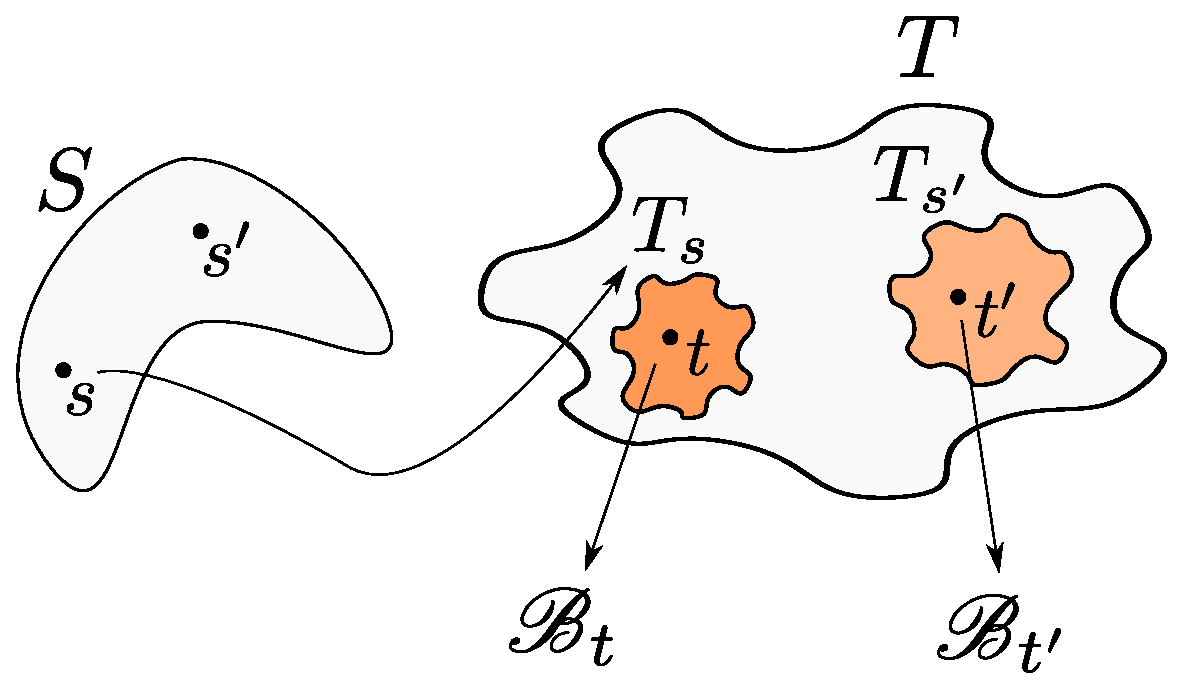
\includegraphics[width=0.7\textwidth]{Figuras/figura-agrupamento-va-idenpendentes.pdf}
\caption{Lema do Agrupamento.}
\label{Rotulo}
\end{figure}
\end{center}
%%%


\begin{lema}[Lema do Agrupamento]
Sejam $T$ um conjunto arbitrário de índices e 
$\{\mathscr{B}_{t},\ t\in T\}$ uma família de 
$\sigma$-álgebras independentes. Seja $S$ 
um conjunto de índices e suponha que 
para cada $s\in S$ temos $T_s\subset T$
e $\{T_s,\ s\in S\}$ seja uma coleção mutuamente disjunta.
Defina 
	\[
		\mathscr{B}_{T_s} 
		=
		\sigma\left(
			\bigcup_{t\in T_s}\mathscr{B}_{t}
		\right).
	\]
Então $\{\mathscr{B}_{T_s},\ s\in S\}$ é uma família 
independente de $\sigma$-álgebras.
\end{lema}



\begin{proof}
Sem perda de generalidade podemos assumir que $S$ é finito. 
Defina 
	\[
		\mathcal{C}_{T_s}
		\equiv
		\left\{
			\bigcap_{t\in K} B_{t}:\
			B_{t}\in\mathscr{B}_{t},\
			K\subset T_s,\
			K\ \text{finito}
		\right\}.
	\]
Por definição temos que $\mathcal{C}_{T_s}$ é um 
$\pi$-sistema para cada $s\in S$ e além do mais 
este $\pi$-sistemas $\{ \mathcal{C}_{T_s}, s\in S\}$ são independentes.

Observe que $\mathcal{C}_{T_s}\subset \mathscr{B}_{T_s}$ 
e por definição de $\sigma$-álgebra gerada que 
$\sigma(\mathcal{C}_{T_s})\subset \mathscr{B}_{T_s}$.
Segue da definição de $\mathcal{C}_{T_s}$, 
tomando $K=\{t\}$, que
para todo $t\in T_s$, é verdadeira a seguinte continência
$\mathscr{B}_{t}\subset \mathcal{C}_{T_s}$. 
Daí segue que $\mathscr{B}_{t}\subset \sigma(\mathcal{C}_{T_s})$,
para todo $t\in T_s$. 
Assim podemos concluir que 
	\[
		\bigcup_{t\in T_s}\mathscr{B}_{t}
		\subset
		\sigma(\mathcal{C}_{T_s}).
	\]
O que implica novamente pela definição de $\sigma$-álgebra
gerada que
	\[
		\mathscr{B}_{T_s}
		\equiv
		\sigma
		\left(
			\bigcup_{t\in T_s}\mathscr{B}_{t}
		\right)		
		\subset
		\sigma(\mathcal{C}_{T_s}).
	\]
Usando a observação do início do paragrafo temos que 
$\sigma(\mathcal{C}_{T_s}) = \mathscr{B}_{T_s}$. Para finalizar 
a prova basta agora aplicar o 
Teorema \ref{teo-criterio-basico-independencia}.
\end{proof}











\section{Lema de Borel Cantelli}

O Lema de Borel-Cantelli é um resultado muito simples 
de ser obtido mas é uma ferramenta básica na obtenção de 
convergência quase certa em várias situações.

\begin{lema}[Lema de Borel-Cantelli]
Sejam $(\Omega,\F,\P)$ um espaço de probabilidade 
e $\{A_n\}$ uma sequência arbitrária de eventos.
Se $\sum_{n=1}^{\infty} \P(A_n)<\infty$ então 
	\[
		\P\left(\limsup_{n\to\infty} A_n\right)=0.
	\]
\end{lema}




\begin{proof}
Usando a definição de $\limsup$, a continuidade de $\P$,
a subaditividade e a hipótese de convergência da série, 
obtemos
	\begin{align*}
	\P\left(\limsup_{n\to\infty} A_n\right)
	&=
	\P\left( \lim_{n\to\infty} \bigcup_{j\geq n} A_j \right)
	\\
	&=
	\lim_{n\to\infty}\P\left( \bigcup_{j\geq n} A_j \right)
	\\
	&\leq
	\limsup_{n\to\infty} \sum_{j=n}^{\infty}\P\left( A_j \right)
	\\
	&=
	0.
	\end{align*}
\end{proof}



\begin{exemplo}
	Suponha que $\{X_n\}$ sejam v.a.'s de Bernoulli 
	com $\P(X_n=1)=p_n=1-\P(X_n=0)$. 
	Observe que não estamos supondo que $\{X_n\}$ é
	uma sequência independente e nem identicamente distribuídas.
	Afirmamos que se $\sum_{n=1}^{\infty}p_n<\infty$ então 
		\[
			\P\left( \lim_{n\to\infty} X_n=0\right)=1. 
		\]
	De fato, se 
		\[
			 \sum_{n=1}^{\infty} \P(X_n=1) 
			 = 
			 \sum_{n=1}^{\infty}p_n 
			 < \infty,
		\]
	então segue do Lema de Borel-Cantelli que $\P(\limsup \{X_n=1\})=0$.
	Tomando complementar ficamos com 
	\[
		1
		=
		\P(\liminf \{X_n=1\}^c)
		=
		\P(\liminf \{X_n=0\}).
	\]
	Por definição do $\liminf$ temos 
	para todo 
	\[
		\omega
		\in 
		\liminf_{n\to\infty} \{X_n=0\}
		=
		\bigcup_{k\geq 1} \bigcap_{n\geq k} \{X_n=0\}		
	\]
	que existe $k=k(\omega)$ tal que 
	$\omega \in \bigcap_{n\geq k(\omega)} \{X_n=0\}$,
	isto é, $X_n(\omega)=0$ para todo $n\geq k(\omega)$
	mostrando que $\lim_{n\to\infty} X_n(\omega)=0$.
	Como este fato vale para $\omega$ em um conjunto 
	de probabilidade um, a afirmação está provada.
\end{exemplo}










